\documentclass[12pt]{exam}

\usepackage{tikz} % Used for Groupwork 7 PHP

% essential packages
\usepackage{fullpage} % margin formatting
\usepackage{enumitem} % configure enumerate and itemize
\usepackage{amsmath, amsfonts, amssymb, mathtools} % math symbols
\usepackage{xcolor, colortbl} % colors, including in tables
\usepackage{makecell} % thicker \Xhline in table
\usepackage{graphicx} % images, resizing

% sometimes needed packages
\usepackage{hyperref} % hyperlinks
% \hypersetup{colorlinks=true, urlcolor=blue}
% \usepackage{logicproof} % natural deduction
% \usepackage{tikz} % drawing graphs
% \usetikzlibrary{positioning}
% \usepackage{multicol}
% \usepackage{algpseudocode} % pseudocode

% paragraph formatting
\setlength{\parskip}{6pt}
\setlength{\parindent}{0cm}

% newline after Solution:
\renewcommand{\solutiontitle}{\noindent\textbf{Solution:}\par\noindent}

% less space before itemize/enumerate
\setlist{topsep=0pt}

% creates \filcl to grey out cells for groupwork grading
\newcommand{\filcl}{\cellcolor{gray!25}}

% creates \probnum to get the problem number
\newcounter{probnumcount}
\setcounter{probnumcount}{1}
\newcommand{\probnum}{\arabic{probnumcount}. \addtocounter{probnumcount}{1}}

% use roman numerals by default
\setlist[enumerate]{label={(\roman*)}}

% creates custom list environments for grading guidelines, question parts
\newlist{guidelines}{itemize}{1}
\setlist[guidelines]{label={}, left=0pt .. \parindent, nosep}
\newlist{gwguidelines}{enumerate}{1}
\setlist[gwguidelines]{label={(\roman*)}, nosep}
\newlist{qparts}{enumerate}{2}
\setlist[qparts]{label={(\alph*)}}
\newlist{qsubparts}{enumerate}{2}
\setlist[qsubparts]{label={(\roman*)}}
\newlist{stmts}{enumerate}{1}
\setlist[stmts]{label={(\roman*)}, nosep}
\newlist{pflist}{itemize}{4}
\setlist[pflist]{label={$\bullet$}, nosep}
\newlist{enumpflist}{enumerate}{4}
\setlist[enumpflist]{label={(\arabic*)}, nosep}

\printanswers

\newcommand{\prevhwnum}{6}
\newcommand{\hwnum}{7}

\begin{document}
%%%%%%%%%%%%%%% TITLE PAGE %%%%%%%%%%%%%%%
\title{EECS 203: Discrete Mathematics\\
  Winter 2024\\
  Homework \hwnum{}}
\date{}
\author{}
\maketitle
\vspace{-50pt}
\begin{center}
  \huge Due \textbf{Thursday, Mar. 21}, 10:00 pm\\
\Large No late homework accepted past midnight.\\
\vspace{10pt}
\large Number of Problems: $8+2$
\hspace{3cm}
Total Points: $100+18$
\end{center}
\vspace{25pt}
\begin{itemize}
    \item \textbf{Match your pages!} Your submission time is when you upload the file, so the time you take to match pages doesn't count against you.
    \item Submit this assignment (and any regrade requests later) on Gradescope. 
    \item Justify your answers and show your work (unless a question says otherwise).
    \item By submitting this homework, you agree that you are in compliance with the Engineering Honor Code and the Course Policies for 203, and that you are submitting your own work.
    \item Check the syllabus for full details.
\end{itemize}
\newpage
%%%%%%%%%%%%%%% TITLE PAGE %%%%%%%%%%%%%%% 

\section*{Individual Portion}

\subsection*{\probnum Growing your Growth Mindset [5 points]}

\begin{qparts}
    \item Watch the linked video about developing a growth mindset. This is a different video than the one you saw in lecture.
    \item Rewrite the last two fixed mindset statements as growth mindset statements.
    \item Write down one of your recurring fixed mindset thoughts, then write a thought you can replace it with that reflects a growth mindset.
\end{qparts}

\textbf{Video:} \href{https://tinyurl.com/eecs203growthMindset}{Developing a Growth Mindset (tinyurl.com/eecs203growthMindset)}

\textbf{What to submit:} Your three pairs of fixed and growth mindset statements 
(the two from the table, and one that you came up with on your own).

\begin{center}
\begin{tabular}{ |p{18em}|p{18em}| } 
\hline
\textbf{Fixed Mindset Statement} & \textbf{Growth Mindset Statement}\\
\hline

When I have to ask for help or get called on in lecture, I get anxious and feel like people will think I’m not smart.

& The question I have is likely the same question someone else in lecture may have. It’s important for me to ask so I can better understand what I am learning.
\\ \hline

I’m jealous of other people’s success.

& I am inspired and encouraged by other people’s success. They show me what is possible.

\\ \hline

I didn’t score as high on the exam as I expected. I’m not going to do well in this class and should drop it.

& I learned from my mistakes on exam 1, and exam 2 will be a new opportunity for me to practice what I’ve learned.

\\ \hline

This class is hard for me, so I am not fit for this major.
& [FILL IN YOUR OWN]
\\ \hline

Either I'm good at Discrete Math, or I'm not. 
& [FILL IN YOUR OWN]
\\ \hline

[FILL IN YOUR OWN] & [FILL IN YOUR OWN] \\ 
\hline
\end{tabular}
\end{center}

\begin{solution}

\end{solution}


\subsection*{\probnum Sketchy Compositions [15 points]}
Consider $f \colon X \to Y $ and $g \colon Y \to X$. \textbf{Prove or disprove} each of the following statements.

\begin{qparts}
    \item If  $ f \circ g $ is one-to-one, then $ g $ must be one-to-one.
    \item If $ g \circ f $ is one-to-one, then $ g $ must be one-to-one.
\end{qparts}

\begin{solution}

\end{solution}

\subsection*{\probnum Flippy Function Fun! [15 points]}

A function $f\colon A\to A$ is said to be \textit{flippy} if for all $a\in A,$ $f(f(a))=a.$ \textbf{Prove or disprove} each of the following statements

\begin{qparts}
    \item If $f\colon A\to A$ is flippy, then $f$ is bijective. (Either prove $f$ is both onto and one-to-one using their respective definitions, or provide a counterexample.)
    \item If $f\colon A\to A$ and $g\colon A\to A$ are flippy, then $f\circ g$ must be flippy.
\end{qparts}

\begin{solution}

\end{solution}


\subsection*{\probnum A Hairy Situation [12 points]}
Assume that nobody on Earth has more than 1,000,000 hairs on their head. Assume that the population of New York City in 2024 is 8,468,000 people. As of 2024, what is the maximum number of people in New York City that we can guarantee all have the same number of hairs on their heads?

Your explanation should use the Pigeonhole Principle. Make sure to state what the pigeons and holes are, as well as how many of each you have. 

\begin{solution}

\end{solution}


\subsection*{\probnum A Pairy Situation [14 points]}
Suppose that $52$ integers are chosen among the set of natural numbers less than $100$. In other words, suppose that $52$ integers are chosen from $\{0 , 1, 2, 3, \dots, 99\}$. \textbf{Prove or disprove} that there must exist at least one pair of integers among those chosen whose difference is equal to 7.

Your proof or disproof should use the Pigeonhole Principle. Make sure to state what the pigeons and holes are, as well as how many of each you have.

\begin{solution}

\end{solution}


\subsection*{\probnum Super Sets [15 points]}
Let $A$ be the set of prime numbers less than $203$. The universe of discourse is $\mathbb{R}$. State whether each of the following sets are empty, finite but nonempty, countably infinite, or uncountable. Briefly justify your answers.

\begin{qparts}
    \item $\mathbb{Z} \times \mathbb{Z}$
    \item $(\mathbb{Z} \times \mathbb{Z}) - (\mathbb{Q} \times \mathbb{Q})$
    \item $\mathbb{R} - \mathbb{Q}$
    \item $\mathbb{Q} - \mathbb{R}$
    \item $A \cap \mathbb{Q}$
    \item $\overline{A} \cap \overline{\mathbb{Q}}$
\end{qparts}

\begin{solution}

\end{solution}


\subsection*{\probnum Cardinal Construction [12 points]}
For each part, give \textit{uncountable} sets $A$ and $B$ such that $A - B$ is
\begin{qparts}
    \item uncountable.
    \item countably infinite.
    \item finite but nonempty.
    \item empty.
\end{qparts}

\begin{solution}

\end{solution}


\subsection*{\probnum Interesting Intervals [12 points]}
Prove that $|[0,3]| = |(2, 5)\cup (6,7)|$. If you construct functions in your solution with certain properties, you may assert that they have those properties without proof.

\begin{solution}

\end{solution}

\pagebreak
\section*{Grading of Groupwork \prevhwnum{}}
Using the solutions and Grading Guidelines, grade your Groupwork \prevhwnum{} Problems:
\begin{itemize}
    \item Use the table below to grade your past Groupwork submission and calculate scores.
    \item While grading, mark up your past submission. Include this with the table when you submit your grading.
    \item Write whether your submission achieved each rubric item. If it didn't achieve one, say why not.
    \item For extra credit, write positive comment(s) about your work.
    \item You don't have to redo problems correctly, but it is recommended!
    \item See ``All About Groupwork" on Canvas for more detailed guidance, and what to do if you change groups.
\end{itemize}

\begin{center}
\resizebox{\textwidth}{!}{\begin{tabular}{| c | c | c | c | c | c | c | c | c | c | c | c | c |}
\hline
 & (i) & (ii) & (iii) & (iv) & (v) & (vi) & (vii) & (viii) & (ix) & (x) & (xi) & Total:\\
\hline
Problem 1 & & & &\filcl &\filcl &\filcl &\filcl &\filcl &\filcl & \filcl& \filcl& \hspace{1cm}/12\\
\hline 
Problem 2 & & & & & & & & &\filcl & \filcl& \filcl& \hspace{1cm}/18\\
\Xhline{1.25pt}
Total: &\filcl &\filcl &\filcl &\filcl &\filcl &\filcl &\filcl &\filcl & \filcl& \filcl& \filcl&\hspace{1cm}/30\\
\hline
\end{tabular}}
\end{center}

\pagebreak
\setcounter{probnumcount}{1}
\section*{Groupwork \hwnum{} Problems}


\subsection*{\probnum Get to the Point [10 points]}
Consider an arbitrary set $A$. We say a function $f:A\rightarrow A$ has a \textit{fixed point} iff there exists $a \in A$ such that $f(a) = a$.

Consider the notation $f^{(n)}$ to mean $\underbrace{f \circ \dots \circ f}_{n \text{ times}}$, where $n \in \mathbb{Z^+}$. Essentially, $n$ copies of $f$ are composed together.

Prove by \textbf{induction} that if $f$ is a function with a fixed point, then for all positive integers $n$, $f^{(n)}$ has a fixed point.

\begin{solution}

\end{solution}


\subsection*{\probnum Going Off the Grid [8 points]}
In a grid, we say that a point $a$ \textit{dominates} a point $b$ iff $a$ lies strictly above and to the right of $b$. For example, in the picture below, $a$ dominates $b$.
\begin{center}
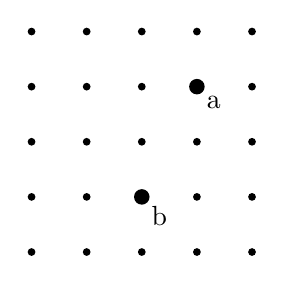
\begin{tikzpicture}[scale=0.7]
  \def\n{5} 
  \foreach \x in {1,...,\n} {
    \foreach \y in {1,...,\n} {
      \ifnum\x=3
        \ifnum\y=2
          \fill (\x,\y) circle (4pt);
          \node[anchor=north west] at (\x,\y) {b};
        \else
          \fill (\x,\y) circle (2pt);
        \fi
      \else
        \ifnum\x=4
          \ifnum\y=4
            \fill (\x,\y) circle (4pt);
            \node[anchor=north west] at (\x,\y) {a};
          \else
            \fill (\x,\y) circle (2pt);
          \fi
        \else
          \fill (\x,\y) circle (2pt);
        \fi
      \fi
    }
  }
\end{tikzpicture}
\end{center}
Prove using the Pigeonhole Principle that if we choose $4n-1$ points from an $n \times n$ grid ($n\ge 4$), there must be three chosen points $x, y, z$ such that $x$ dominates $y$ and $y$ dominates $z$. Make sure to state what your pigeons are and what your holes are, as well as how many of each you have.

\textbf{Hint:} If $x, y, z$ lie on the same increasing diagonal as shown in the picture below, then $x$ dominates $y$ and $y$ dominates $z$.
\begin{center}
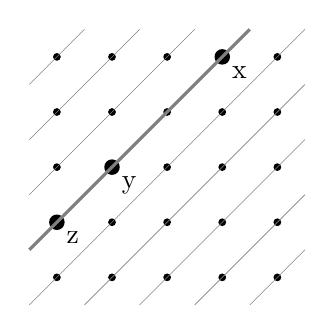
\begin{tikzpicture}[scale=0.7]
  \def\n{5}
  \foreach \x in {1,...,\n} {
    \foreach \y in {1,...,\n} {
      \ifnum\x=4
        \ifnum\y=5
          \fill (\x,\y) circle (4pt);
          \node[anchor=north west] at (\x,\y) {x};
        \else
          \fill (\x,\y) circle (2pt);
        \fi
      \else
        \ifnum\x=2
          \ifnum\y=3
            \fill (\x,\y) circle (4pt);
            \node[anchor=north west] at (\x,\y) {y};
          \else
            \fill (\x,\y) circle (2pt);
          \fi
        \else
          \ifnum\x=1
            \ifnum\y=2
              \fill (\x,\y) circle (4pt);
              \node[anchor=north west] at (\x,\y) {z};
            \else
              \fill (\x,\y) circle (2pt);
            \fi
          \else
            \fill (\x,\y) circle (2pt);
          \fi
        \fi
      \fi
    }
  }

  
  \draw [very thin, gray] (0.5, 4.5) -- (1.5, 5.5);
  \draw [very thin, gray] (0.5, 3.5) -- (2.5, 5.5);
  \draw [very thin, gray] (0.5, 2.5) -- (3.5, 5.5);
  \draw [very thick, gray] (0.5, 1.5) -- (4.5, 5.5);
  \draw [very thin, gray] (0.5, 0.5) -- (5.5, 5.5);
  \draw [very thin, gray] (1.5, 0.5) -- (5.5, 4.5);
  \draw [very thin, gray] (2.5, 0.5) -- (5.5, 3.5);
  \draw [very thin, gray] (3.5, 0.5) -- (5.5, 2.5);
  \draw [very thin, gray] (4.5, 0.5) -- (5.5, 1.5);

\end{tikzpicture}
\end{center}

\begin{solution} 

\end{solution}

\end{document}
